Plot~\ref{pgfplot:20130523} shows ...
\begin{figure}
  \caption{Atomic broadcast on gruyere with tree (red) and
    cluster(blue) topology}
  \label{pgfplot:20130523}
  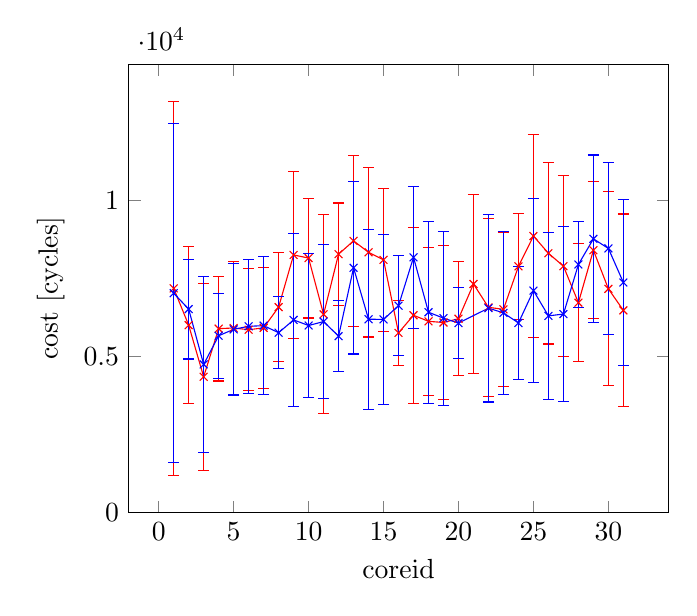
\begin{tikzpicture}
    \begin{axis}[
        xlabel={coreid},
        ylabel={cost [cycles]}
        ]
    \addplot[
        color=red,
        mark=x,
        error bars/y dir=both,
        error bars/y explicit
        ] coordinates {
      (1,7191.200000) +- (5989.150370,5989.150370)
      (2,6011.800000) +- (2523.104746,2523.104746)
      (3,4356.300000) +- (3005.000101,3005.000101)
      (4,5899.200000) +- (1679.566658,1679.566658)
      (5,5920.900000) +- (2138.061807,2138.061807)
      (6,5864.600000) +- (1954.012293,1954.012293)
      (7,5924.900000) +- (1941.433514,1941.433514)
      (8,6589.700000) +- (1750.721854,1750.721854)
      (9,8262.500000) +- (2664.882146,2664.882146)
      (10,8162.500000) +- (1920.496876,1920.496876)
      (11,6358.500000) +- (3187.482525,3187.482525)
      (12,8288.400000) +- (1639.762373,1639.762373)
      (13,8713.400000) +- (2735.916636,2735.916636)
      (14,8347.800000) +- (2717.770991,2717.770991)
      (15,8104.600000) +- (2299.087088,2299.087088)
      (16,5765.200000) +- (1039.328322,1039.328322)
      (17,6329.000000) +- (2825.671389,2825.671389)
      (18,6134.100000) +- (2368.037096,2368.037096)
      (19,6096.500000) +- (2463.720774,2463.720774)
      (20,6217.600000) +- (1828.323943,1828.323943)
      (21,7331.200000) +- (2861.751240,2861.751240)
      (22,6583.300000) +- (2856.719379,2856.719379)
      (23,6518.200000) +- (2465.511947,2465.511947)
      (24,7897.300000) +- (1693.680492,1693.680492)
      (25,8868.200000) +- (3245.564043,3245.564043)
      (26,8316.000000) +- (2910.331012,2910.331012)
      (27,7902.900000) +- (2893.679749,2893.679749)
      (28,6731.800000) +- (1897.894454,1897.894454)
      (29,8414.400000) +- (2190.628412,2190.628412)
      (30,7175.900000) +- (3113.089123,3113.089123)
      (31,6484.600000) +- (3091.445623,3091.445623)
    };

    \addplot[
        color=blue,
        mark=x,
        error bars/y dir=both,
        error bars/y explicit
        ] coordinates {
      (1,7035.600000) +- (5432.187298,5432.187298)
      (2,6527.000000) +- (1599.367625,1599.367625)
      (3,4752.100000) +- (2817.137925,2817.137925)
      (4,5672.600000) +- (1360.118098,1360.118098)
      (5,5876.800000) +- (2103.412836,2103.412836)
      (6,5974.700000) +- (2143.240213,2143.240213)
      (7,5995.500000) +- (2216.524949,2216.524949)
      (8,5769.500000) +- (1155.924760,1155.924760)
      (9,6179.000000) +- (2781.637719,2781.637719)
      (10,6000.000000) +- (2296.150823,2296.150823)
      (11,6125.700000) +- (2471.338465,2471.338465)
      (12,5658.400000) +- (1139.523163,1139.523163)
      (13,7850.700000) +- (2764.155424,2764.155424)
      (14,6201.200000) +- (2886.178054,2886.178054)
      (15,6196.500000) +- (2731.240240,2731.240240)
      (16,6636.200000) +- (1596.941627,1596.941627)
      (17,8185.900000) +- (2274.981250,2274.981250)
      (18,6426.400000) +- (2912.780259,2912.780259)
      (19,6234.800000) +- (2789.759051,2789.759051)
      (20,6078.000000) +- (1143.030008,1143.030008)
      (22,6556.700000) +- (3007.839958,3007.839958)
      (23,6405.200000) +- (2622.700928,2622.700928)
      (24,6080.900000) +- (1820.274674,1820.274674)
      (25,7119.300000) +- (2958.161221,2958.161221)
      (26,6309.000000) +- (2668.378197,2668.378197)
      (27,6367.100000) +- (2804.061249,2804.061249)
      (28,7957.600000) +- (1379.318324,1379.318324)
      (29,8778.100000) +- (2688.111473,2688.111473)
      (30,8471.700000) +- (2767.067041,2767.067041)
      (31,7378.300000) +- (2658.470502,2658.470502)
    };

    \end{axis}
  \end{tikzpicture}
\end{figure}
